
\documentclass[10pt]{beamer}\usepackage[]{graphicx}\usepackage[]{xcolor}
% maxwidth is the original width if it is less than linewidth
% otherwise use linewidth (to make sure the graphics do not exceed the margin)
\makeatletter
\def\maxwidth{ %
  \ifdim\Gin@nat@width>\linewidth
    \linewidth
  \else
    \Gin@nat@width
  \fi
}
\makeatother

\definecolor{fgcolor}{rgb}{0.345, 0.345, 0.345}
\newcommand{\hlnum}[1]{\textcolor[rgb]{0.686,0.059,0.569}{#1}}%
\newcommand{\hlstr}[1]{\textcolor[rgb]{0.192,0.494,0.8}{#1}}%
\newcommand{\hlcom}[1]{\textcolor[rgb]{0.678,0.584,0.686}{\textit{#1}}}%
\newcommand{\hlopt}[1]{\textcolor[rgb]{0,0,0}{#1}}%
\newcommand{\hlstd}[1]{\textcolor[rgb]{0.345,0.345,0.345}{#1}}%
\newcommand{\hlkwa}[1]{\textcolor[rgb]{0.161,0.373,0.58}{\textbf{#1}}}%
\newcommand{\hlkwb}[1]{\textcolor[rgb]{0.69,0.353,0.396}{#1}}%
\newcommand{\hlkwc}[1]{\textcolor[rgb]{0.333,0.667,0.333}{#1}}%
\newcommand{\hlkwd}[1]{\textcolor[rgb]{0.737,0.353,0.396}{\textbf{#1}}}%
\let\hlipl\hlkwb

\usepackage{framed}
\makeatletter
\newenvironment{kframe}{%
 \def\at@end@of@kframe{}%
 \ifinner\ifhmode%
  \def\at@end@of@kframe{\end{minipage}}%
  \begin{minipage}{\columnwidth}%
 \fi\fi%
 \def\FrameCommand##1{\hskip\@totalleftmargin \hskip-\fboxsep
 \colorbox{shadecolor}{##1}\hskip-\fboxsep
     % There is no \\@totalrightmargin, so:
     \hskip-\linewidth \hskip-\@totalleftmargin \hskip\columnwidth}%
 \MakeFramed {\advance\hsize-\width
   \@totalleftmargin\z@ \linewidth\hsize
   \@setminipage}}%
 {\par\unskip\endMakeFramed%
 \at@end@of@kframe}
\makeatother

\definecolor{shadecolor}{rgb}{.97, .97, .97}
\definecolor{messagecolor}{rgb}{0, 0, 0}
\definecolor{warningcolor}{rgb}{1, 0, 1}
\definecolor{errorcolor}{rgb}{1, 0, 0}
\newenvironment{knitrout}{}{} % an empty environment to be redefined in TeX

\usepackage{alltt}

\usepackage{xcolor}
\usepackage{mathtools}
\usepackage{graphicx} 
\usepackage{amsmath}
\usepackage{listings}

\usepackage{color}
\newcommand{\vet}[1]{{\ensuremath{\mbox{\boldmath $#1$}}}}
\definecolor{groen}{rgb}{0.0,0.9,0.0}

\lstnewenvironment{rc}[1][]{\lstset{language=R}}{}

\graphicspath{{images/}}
\usepackage{tikz} 
\usetikzlibrary{arrows,calc,patterns,positioning,shapes,decorations.markings} 
\usetikzlibrary{decorations.pathmorphing} 

%\usetheme{default}
\mode<presentation>
{
	\usetheme{Singapore}
	\usecolortheme{crane}
	% or ...
	
	\setbeamercovered{transparent}
	% or whatever (possibly just delete it)
}

\title{Introduction to Structural Equation Modeling using lavaan}
\subtitle{Model Selection}
\author{R. M. Kuiper}
\institute{Department of Methodology \& Statistics \\ Utrecht University}
\date{}

%------------------------------------------------------------------------------%
%\hypersetup{bookmarksopen=false}
\hypersetup{bookmarksdepth=-2}
\AtBeginSection[]
{
    \begin{frame}
        \frametitle{Table of Contents}
        \tableofcontents[currentsection] %subsectionstyle=hide] %, hidesubsections]
    \end{frame}
}
\IfFileExists{upquote.sty}{\usepackage{upquote}}{}
\begin{document}
%\SweaveOpts{concordance=TRUE}


%------------------------------------------------------------------------------%

\begin{frame}[t, plain]
  \titlepage
\end{frame}
%------------------------------------------------------------------------------%
%
%------------------------------------------------------------------------------%
%
\begin{frame}[fragile]{\textit{Previously:} Model Comparisons: AIC / BIC}

Suitable for comparing
\begin{itemize}
  \item both nested and non-nested models/hypotheses.
  \item more than two models/hypotheses.
\end{itemize}

\vspace*{5mm}

Choose the model/hypothesis with the \textcolor{red}{lowest} AIC and/or BIC.

\vspace*{5mm}

To be discussed in the Model Selection lecture
\begin{itemize}
  \item Quantify relative support via IC weights.\\
\begin{knitrout}
\definecolor{shadecolor}{rgb}{0.969, 0.969, 0.969}\color{fgcolor}\begin{kframe}
\begin{alltt}
\hlkwd{library}\hlstd{(devtools)} \hlcom{# Make sure you have Rtools}
\hlkwd{install_github}\hlstd{(}\hlstr{"rebeccakuiper/ICweights"}\hlstd{)}
\hlkwd{library}\hlstd{(ICweights)}
\hlopt{?}\hlstd{IC.weights}
\end{alltt}
\end{kframe}
\end{knitrout}
  \item Extension AIC for order-restricted hypotheses \\ (GORIC and GORICA).\\
\begin{knitrout}
\definecolor{shadecolor}{rgb}{0.969, 0.969, 0.969}\color{fgcolor}\begin{kframe}
\begin{alltt}
\hlkwd{library}\hlstd{(restriktor)}
\hlkwd{library}\hlstd{(goric)}
\end{alltt}
\end{kframe}
\end{knitrout}
\end{itemize}

\end{frame}
%------------------------------------------------------------------------------%
%
\begin{frame}{Outline of this lecture}
\tableofcontents[hidesubsections]
\end{frame}
%------------------------------------------------------------------------------%
%
%------------------------------------------------------------------------------%
\section{IC}
%------------------------------------------------------------------------------%
%
%------------------------------------------------------------------------------%
%
\begin{frame}
	\frametitle{Why information criteria?}
	Why do we need information criteria?
	\begin{itemize}
		\item to compare \textbf{non-nested} models/hypotheses.
		%\pause
		\item to compare \textbf{more than two} models at the time.
		%\pause
		\item because there are \textbf{different ideas} about what poses a good model.
	\end{itemize}
	
\end{frame}
%------------------------------------------------------------------------------%
%
\begin{frame}
	\frametitle{Model selection using information criteria}
	
	Describe data as good as possible (fit) \\
  with fewest number of parameters (simplicity / non-complexity).
	
	\bigskip
	
	\begin{block}{General form of information criteria:}
		\bigskip
		{\centerline{
				\textbf{model misfit + model complexity}}
		}
	\end{block}

	\bigskip
	Model/Hypothesis with the \textbf{smallest value} is considered the best model.
\end{frame}
%------------------------------------------------------------------------------%
%
\begin{frame}
	\frametitle{AIC}
	
	\centerline{	IC = \textbf{{\color{orange}{model misfit}} + {\color{purple}{model complexity}}}}
	\vspace{.5 cm}
	
	{\textbf{AIC}: minimize the \textbf{Kullback-Leibler distance}}

	\vspace{1cm}
	\centerline{{\textbf{AIC} ={\color{orange}{ $\;-2\log f(y|\hat{\theta}_y)$}} + \color{purple}{$2 p$}}}
	
	\vspace{.5 cm}
	where $\hat{\theta}_y$ is the maximum likelihood estimate.
	
\end{frame}
%------------------------------------------------------------------------------%
%
\begin{frame}
	\frametitle{Intermezzo: Kullback-Leibler (K-L) distance}

		The K-L distance quantifies the distance between
		\begin{itemize}
			\item the \textbf{truth}: $p(\cdot)$
			\item the \textbf{model under consideration}: $f(\cdot|\theta)$\\
		\end{itemize}
		
		\vspace{.5 cm}
		
		Extra:\\
		\centerline{ K-L = {$\mathrm{E}_{p(y)}\Bigl[\log p(y) -
		\log f(y|\theta)\Bigr]$}}
    \bigskip
			
		% \begin{block}{Remarks}
		% 	\begin{itemize}
		% 		\item minimize K-L. 
		% 		\item Between models, $p(y)$ is constant and can be ignored.
		% 		\item Since $\log f(y|\theta) \geq 0$, maximize $\mathrm{E}[\log f(y|\theta)]$.
		% 		\item AIC: use $\hat{\theta}_y$ as an estimate for $\theta$.
		% 		\item Overfitting: since $y$ is used both to evaluate $f(y|\cdot)$ and compute $\hat{\theta}_y$.
		% 		\\ In the limit, $p$ corrects for overfitting.
		% 	\end{itemize}
		% \end{block}
				
\end{frame}
%------------------------------------------------------------------------------%
%
\begin{frame}
	\frametitle{Alternative to AIC: BIC}
	
	\centerline{	IC = \textbf{{\color{orange}{model misfit}} + {\color{purple}{model complexity}}}}
	
	\vspace{1 cm}
	{\textbf{BIC}:
		maximize the \textbf{marginal model probability} (cf. Bayes Factor)}
	
	\vspace{.5 cm}
	\centerline{{\textbf{BIC} ={\color{orange}{$\;-2\log f(y|\hat{\theta}_y)$}} + \color{purple}{$\log(n) p $}}}
	
	\vspace{.5 cm}
	where $\hat{\theta}_y$ is the maximum likelihood estimate.
	
	\vspace{.5 cm}
	\begin{block}{Note:}
		Difference in penalty AIC vs BIC: $2 p$ vs $\log(n) p$.\\
		(due to different derivation)
	\end{block}
	 
\end{frame}
%------------------------------------------------------------------------------%
%
\begin{frame}
	\frametitle{Order-restricted generalization of AIC: GORIC}
	
	\centerline{	IC = \textbf{{\color{orange}{model misfit}} + {\color{purple}{model complexity}}}}
	\vspace{.5 cm}
	
	{\textbf{GORIC}: minimize the \textbf{K-L distance}}
	
	\vspace{1cm}
	\centerline{{\textbf{GORIC} ={\color{orange}{ $\;-2\log f(y|\tilde{\theta}_y)$}} + \color{purple}{$2 PT$}}}
	
	\vspace{.5 cm}
	where $\tilde{\theta}_y$ is the order-restricted maximum likelihood estimate and\\
	$PT$ can be seen as the expected number of distinct parameters.
	
	\vspace{.5 cm}
	\footnotesize{
	Kuiper, R.M., Hoijtink, H. and Silvapulle, M.J. (2011). An Akaike type information criterion for model selection under inequality constraints. \emph{Biometrika, 98}, 495-501.
	}
	
\end{frame}
%------------------------------------------------------------------------------%
%
\begin{frame}{Intermezzo: Idea penalty (PT)}{loose interpretation}
\begin{displaymath}
H_1: \mu_1 > \mu_2 > \mu_3
\end{displaymath}
contains 1 ordering of three means, 1-2-3. \\
Thus, not complex (i.e., parsimonious).
\begin{displaymath}
H_2: \mu_1 > \mu_2, \mu_3
\end{displaymath}
contains 2 orderings of three means: 1-2-3 and 1-3-2. \\
Thus, more complex (less parsimonious).
\begin{displaymath}
H_u: \mu_1 , \mu_2 , \mu_3
\end{displaymath}
contains all six possible orderings of three means. \\
Thus, is most complex one (not parsimonious).
\end{frame}
%------------------------------------------------------------------------------%
%
\begin{frame}
	\frametitle{GORIC Approximation: GORICA}
	
	\centerline{	IC = \textbf{{\color{orange}{model misfit}} + {\color{purple}{model complexity}}}}
	\vspace{.5 cm}
	
	{\textbf{GORICA}: Approximate GORIC, thus minimize the \textbf{K-L distance}}
	
	\vspace{0.5cm}
	\centerline{{\textbf{GORICA} ={\color{orange}{ $\;-2\log f(\hat{\theta}, \hat{\Sigma}_{\theta}|\tilde{\theta})$}} + \color{purple}{$2 PT$}}}
	
	\vspace{.5 cm}
	
	where 
	\begin{itemize}
			\item $\hat{\theta}$ are the parameters of the unconstrained model,
			\item $\hat{\Sigma}_{\theta}$ is the variance matrix of $\hat{\theta}$,
			%\item $\hat{\theta}, \hat{\Sigma}_{\theta}$ summarize the data (cf. $y$ in the GORIC),
			\item $\tilde{\theta}$ is the order-restricted maximum likelihood estimate, and
			\item $PT$ can be seen as the expected number of distinct parameters. %(same as in GORIC).
		\end{itemize}
		
\vspace{.5 cm}

	\footnotesize{
	Alt{\i}n{\i}\c{s}{\i}k, Y., Van Lissa, C. J., Hoijtink, H., Oldehinkel, A. J., and Kuiper, R. M. (2021). Evaluation of inequality constrained hypotheses using a generalization of the AIC. \emph{Psychological Methods}, 26(5), 599-621. %\url{https://doi.org/10.1037/met0000406}
	}
	
\end{frame}
%------------------------------------------------------------------------------%
%
\begin{frame}
	\frametitle{GORICA vs GORIC}
	
	Similarities with GORIC:
		\begin{itemize}
			\item Form: $-2 \ fit + 2 \ complexity$.
			\item Broad type of restrictions.
		\end{itemize}
		
		\vspace{.5 cm}
	
	Differences compared to GORIC:
		\begin{itemize}
			\item Uses asymptotic expression of the likelihood (is a normal): \\
			can therefore be easily applied to all types of statistical models. \\
			Disadvantage: might work less well in case of small samples.
			\item Does not need data set, but
			mle's and their covariance matrix.
			\item Can leave out nuisance parameters (i.e., not part of hypotheses).
		\end{itemize}
	
	\vspace{.5 cm}
	
	Note:\\
		In case of normal linear models and/or not too small samples: \\
		GORICA weights = GORIC weights.
\end{frame}
%------------------------------------------------------------------------------%
%
\begin{frame}
	\frametitle{Why GORIC and GORICA?}

Most researchers have a-priori ``order-restricted'' / ``informative'' / ``theory-based'' hypotheses, e.g.:

\vspace{.5 cm}

$H_{1}:  \mu_1 > \mu_2 > \mu_3$ (in an ANOVA model) or \\
$H_{1}:  \beta_1 > \beta_2 > \beta_3 > \beta_4$ (in a regression/SEM model). 
%since they are expert in their research field.

\vspace{2\baselineskip}
\includegraphics[width = 0.6\linewidth]{Model-Unc.png}
%\vspace{\baselineskip}

\end{frame}
%------------------------------------------------------------------------------%
%
\begin{frame}
	\frametitle{Note on comparable estimates}
	
	\begin{block}{Continuous predictors}
		If compare relative strength/importance of parameters (e.g., $\beta_1 > \beta_2$), \\ 
		then make sure comparable: \\
		e.g., standardize continuous predictors.
	\end{block}
	~\\
	
	\begin{block}{Multiple outcomes}
		If compare parameters across outcomes, \\ 
		then (also) standardize outcomes.
	\end{block}
	
\end{frame}
%------------------------------------------------------------------------------%
%
\begin{frame}{Note on including ``unconstrained'' hypothesis}%{Highest fit but also most complex, thus failsafe}
If set of hypotheses does not contain a reasonable/good one:\\
Select the best of set of weak hypotheses.
% Aarde is plat
% Aarde is pyramide
% Kiezen dan laatste, nl 2e is beter dan 1e, maar wil je niet.
% Als ook Hunc (is no structure), then you will choose that one!

\vspace{-0.5\baselineskip}
\begin{block}{}
Prevent choosing a weak hypothesis \\
by including unconstrained hypothesis $H_u$ (or $H_a$):
\begin{eqnarray}
\nonumber H_0: && \mu_1 = \mu_2 = \mu_3,\\
\nonumber H_1: && \mu_1 > \mu_2 > \mu_3,\\
\nonumber H_u: && \mu_1, \mu_2, \mu_3, \\
\nonumber && \mbox{(i.e., \textit{no restrictions})}.
\end{eqnarray}
$H_u$ highest fit but also most complex, thus failsafe.
\end{block}

\vspace{0.5\baselineskip}
Note: GORIC for $H_0$ and $H_u$ equals AIC value.	
\end{frame}
%------------------------------------------------------------------------------%
%
\begin{frame}
\frametitle{Confirmation more power: 1 data set. GORIC values for $3$ groups, effect size $ES$, and $\mathbf{n=10}$ observations per group}
%%In Figure~\ref{GORICvsAIC}, the GORIC values are given for these three hypotheses (for $n = 10$ and $n = 100$).
%The GORIC reduces to the Akaike information criterion (AIC) when there are no order restrictions, that is, for hypotheses $H_0$ and $H_a$.
%%The GORIC values for $H_0$ increase with $ES$, because the differences between the sample means
%%$\overline{y}_i$ and the restricted means $\hat{\mu}_{0i} = \overline{\mu}_0$ (for $i = 1, \ldots, k$) increase with increasing effect size.
%%This leads to a decrease in the log likelihood (see (\ref{LogLik})) and, consequently, an increase in GORIC value (see (\ref{GORIC})).
%%The GORIC values for $H_1$ and $H_a$ do not depend on effect size, since the sample means are in accordance with $H_1$ and, logically, $H_a$.
%%So, the difference between
%%$\overline{y}_i$ and $\hat{\mu}_{mi}$ (for $i = 1, \ldots, k$) is zero for both $H_1$ and $H_a$ for each effect size.
%%This implies that the likelihood values for $H_1$ and $H_a$ are equal, therefore, the difference in GORIC values equals two times the difference in the penalty terms, that is,
%%$2 (PT_2 - PT_1) = 2 (4 - 2 \frac{5}{6}) = 2 \frac{1}{3}$.
%When the sample means are in accordance with $H_1$, $H_1$ is always preferred over $H_a$, because of lower 'penalty'.
%
%Compared to $H_a$, $H_1$ will be preferred over $H_0$ for smaller effect sizes.
%This implies that the probability of choosing the correct/best hypothesis is higher if $H_0$ is compared to $H_1$ than if $H_0$ is compared to $H_a$ (when $H_1$ is true).
%
\begin{figure}
    \centering
  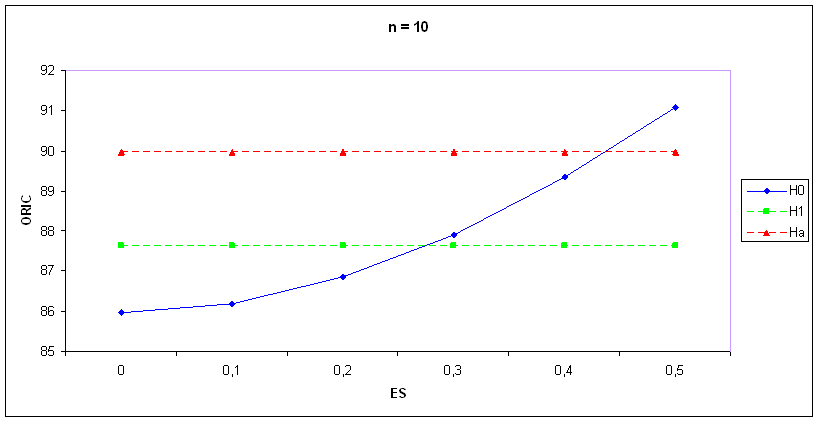
\includegraphics[scale = 0.54]{ORICvsAIC_n10.png}\\
%  \caption{GORIC values for one generated data set with $3$ groups, effect size $ES$, and $n$ observations per group}
\end{figure}

\end{frame}
%------------------------------------------------------------------------------%
%
\begin{frame}
\frametitle{Confirmation more power: 1 data set. GORIC values for $3$ groups, effect size $ES$, and $\mathbf{n=100}$ observations per group}
\begin{figure}
    \centering
  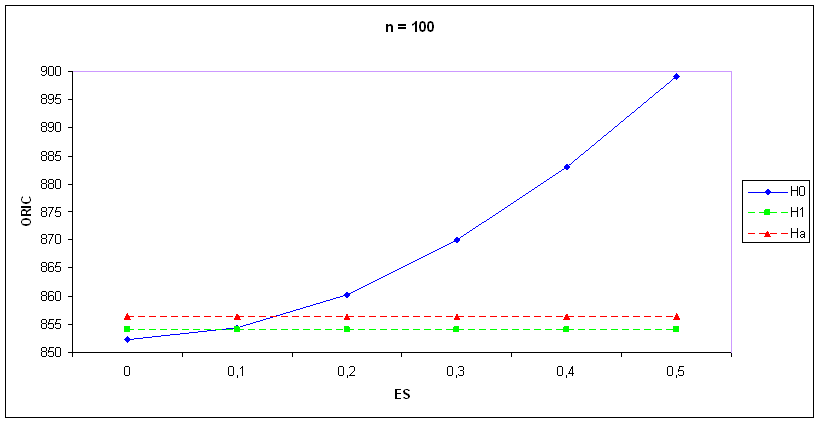
\includegraphics[scale = 0.54]{ORICvsAIC_n100.png}\\
%  \caption{GORIC values for one generated data set with $3$ groups, effect size $ES$, and $n$ observations per group}
\end{figure}

\end{frame}
%------------------------------------------------------------------------------%
%
\begin{frame}{Note on hypotheses}
	\begin{enumerate}
		\item Only include hypotheses with sound theoretical and/or empirical basis.\\
		Note: Often a null hypothesis is not of interest.
		\item Keep the number of hypotheses included as small as possible.
		\item This is indeed a subjective endeavor, aim for inter-peer / inter-subjective agreement.
	\end{enumerate}
\end{frame}

%------------------------------------------------------------------------------%
%
%------------------------------------------------------------------------------%
\section{AIC in R}
%------------------------------------------------------------------------------%
%
%------------------------------------------------------------------------------%
%
\begin{frame}{Example: Multigroup regression}

Regression example from lab meeting `Intro and regression' and `Multigroup analysis' lecture:
\begin{itemize}
  \item{Outcome: sw}
  \item{Predictors: overt and covert}
  \item{Group: gender (males and females)}
\end{itemize}
          
\end{frame}
%------------------------------------------------------------------------------%
%
\begin{frame}[fragile]{Example: Multigroup regression - data}

\begin{knitrout}
\definecolor{shadecolor}{rgb}{0.969, 0.969, 0.969}\color{fgcolor}\begin{kframe}
\begin{alltt}
\hlcom{# Data}
\hlstd{data_regr} \hlkwb{<-} \hlkwd{read.table}\hlstd{(}\hlstr{"popular_regr.txt"}\hlstd{,} \hlkwc{header} \hlstd{= T)}

\hlstd{data_regr[}\hlkwd{sapply}\hlstd{(data_regr,} \hlkwa{function}\hlstd{(}\hlkwc{x}\hlstd{)}
          \hlkwd{as.character}\hlstd{(x)} \hlopt \hlkwd{c}\hlstd{(}\hlstr{"-99"}\hlstd{,} \hlstr{"-999"}\hlstd{) )]} \hlkwb{<-} \hlnum{NA}

\hlstd{data_regr}\hlopt{$}\hlstd{gender} \hlkwb{<-} \hlkwd{factor}\hlstd{(data_regr}\hlopt{$}\hlstd{gender,}
                           \hlkwc{labels} \hlstd{=} \hlkwd{c}\hlstd{(}\hlstr{"male"}\hlstd{,} \hlstr{"female"}\hlstd{))}
\end{alltt}
\end{kframe}
\end{knitrout}
          
\end{frame}
%------------------------------------------------------------------------------%
%
\begin{frame}[fragile]{Example: Multigroup regression - model specification}

\begin{knitrout}
\definecolor{shadecolor}{rgb}{0.969, 0.969, 0.969}\color{fgcolor}\begin{kframe}
\begin{alltt}
\hlcom{# Model specification}

\hlcom{# Model 1}
\hlstd{model.MGregr} \hlkwb{<-} \hlstr{'
  sw ~ overt + covert # regression
  sw ~~ sw            # residual variance
  sw ~ 1              # intercept
'}

\hlcom{# Model 2}
\hlstd{model.MGregr_equal} \hlkwb{<-} \hlstr{'
  # model with labeled parameters
  sw ~ c(b1,b1)*overt + c(b2,b2)*covert 
  sw ~~ sw                                      
  sw ~ 1                                        
'}
\end{alltt}
\end{kframe}
\end{knitrout}
          
\end{frame}
%------------------------------------------------------------------------------%
%
\begin{frame}[fragile]{Example: Multigroup regression - fitting model}

\begin{knitrout}
\definecolor{shadecolor}{rgb}{0.969, 0.969, 0.969}\color{fgcolor}\begin{kframe}
\begin{alltt}
\hlcom{# Fit model}

\hlcom{# Model 1}
\hlstd{fit_MGregr} \hlkwb{<-} \hlkwd{lavaan}\hlstd{(}\hlkwc{model} \hlstd{= model.MGregr,}
                    \hlkwc{data} \hlstd{= data_regr,}
                    \hlkwc{group} \hlstd{=} \hlstr{"gender"}\hlstd{)} \hlcom{# multigroup}

\hlcom{# Model 2}
\hlstd{fit_MGregr_equal} \hlkwb{<-} \hlkwd{lavaan}\hlstd{(}\hlkwc{model} \hlstd{= model.MGregr_equal,}
                    \hlkwc{data} \hlstd{= data_regr,}
                    \hlkwc{group} \hlstd{=} \hlstr{"gender"}\hlstd{)} \hlcom{# multigroup}
\end{alltt}
\end{kframe}
\end{knitrout}
          
\end{frame}
%------------------------------------------------------------------------------%
%
\begin{frame}[fragile]{Example: Multigroup regression - Alternative specification}

\begin{knitrout}
\definecolor{shadecolor}{rgb}{0.969, 0.969, 0.969}\color{fgcolor}\begin{kframe}
\begin{alltt}
\hlstd{model.MGregr_unequal} \hlkwb{<-} \hlstr{'
  # model with labeled parameters
  sw ~ c(b1_m,b1_f)*overt + c(b2_m,b2_f)*covert 
  sw ~~ sw                                      
  sw ~ 1                                        
'}

\hlcom{# Model 1}
\hlstd{fit_MGregr} \hlkwb{<-} \hlkwd{lavaan}\hlstd{(}\hlkwc{model} \hlstd{= model.MGregr_unequal,}
                    \hlkwc{data} \hlstd{= data_regr,}
                    \hlkwc{group} \hlstd{=} \hlstr{"gender"}\hlstd{)} \hlcom{# multigroup}

\hlcom{# Model 2}
\hlstd{fit_MGregr_equal} \hlkwb{<-} \hlkwd{lavaan}\hlstd{(}\hlkwc{model} \hlstd{= model.MGregr_unequal,}
                    \hlkwc{data} \hlstd{= data_regr,}
                    \hlkwc{group} \hlstd{=} \hlstr{"gender"}\hlstd{,} \hlcom{# multigroup}
                    \hlkwc{constraints} \hlstd{=} \hlkwd{c}\hlstd{(}\hlstr{"b1_m == b1_f; 
                                    b2_m == b2_f"}\hlstd{))}
\end{alltt}
\end{kframe}
\end{knitrout}
          
\end{frame}
%------------------------------------------------------------------------------%
%
\begin{frame}[fragile]{Example: Multigroup regression - model comparison}

\begin{knitrout}
\definecolor{shadecolor}{rgb}{0.969, 0.969, 0.969}\color{fgcolor}\begin{kframe}
\begin{alltt}
\hlcom{# Compare models, }
\hlcom{# i.e., evaluate equality of regression coefficients,}
\hlcom{# using AIC}

\hlcom{#anova(fit_MGregr, fit_MGregr_equal)[1:2] }
\hlcom{# or}
\hlkwd{AIC}\hlstd{(fit_MGregr, fit_MGregr_equal)}
\end{alltt}
\begin{verbatim}
##                  df      AIC
## fit_MGregr        8 2319.833
## fit_MGregr_equal  6 2316.868
\end{verbatim}
\end{kframe}
\end{knitrout}

Model with equality constraints has lowest AIC, so is preferred.\\
But how much?

\end{frame}
%------------------------------------------------------------------------------%
%
%------------------------------------------------------------------------------%
%
\begin{frame}[fragile]{Example: Multigroup regression - model comparison}

AIC for n = 100 vs n = 1491: % dim(data_regr)[1]



\begin{knitrout}
\definecolor{shadecolor}{rgb}{0.969, 0.969, 0.969}\color{fgcolor}\begin{kframe}
\begin{alltt}
\hlkwd{round}\hlstd{(AIC_n,} \hlnum{3}\hlstd{)}
\end{alltt}
\begin{verbatim}
##                  AIC_n100 AIC_n1491
## fit_MGregr        125.170  2319.833
## fit_MGregr_equal  124.309  2316.868
## abs. diff.          0.861     2.965
\end{verbatim}
\end{kframe}
\end{knitrout}

AIC increases with sample size.\\
Absolute difference in AIC values also increases.\\

\vspace{\baselineskip}

Model with equality constraints has lowest AIC, so is preferred.\\
But how much?

\end{frame}
%------------------------------------------------------------------------------%
%
%------------------------------------------------------------------------------%
\section{IC weights}
%------------------------------------------------------------------------------%
%
%------------------------------------------------------------------------------%
%
\begin{frame}[fragile]{IC vs IC weights}
	
	IC values:\\ 
	Cannot be interpreted, only compared: smallest is best.
	
	\vspace{\baselineskip}
	
	IC weights ($\mathit{w_{m}}$): \\
	$-$ $\mathit{w_{m}}$: quantifies how much more $H_m$ is supported than others in set.\\ 
	$-$ $\mathit{w_{m}}$/$\mathit{w_{m'}}$: quantifies relative support of $H_m$ vs $H_{m'}$.\\
	Note: The bigger, the better.
	
	\vspace{\baselineskip}
	
	Extra:\\
		$\mathit{w_{m}} = \frac{exp(-0.5~IC_m)}{\sum_{m'=1}^{M}exp(-0.5~IC_{m'})}$.
	
	\vspace{\baselineskip}
	
	\footnotesize{
		Reference:\\
		Kuiper, R.M., Hoijtink, H. and Silvapulle, M.J. (2012). Generalization of the order restricted information criterion for multivariate normal linear models. \emph{Journal of Statistical Planning and Inference, 142}, 2454-2463.
	}
\end{frame}
%------------------------------------------------------------------------------%
%
\begin{frame}[fragile]{IC weights: Interpretation}
	
	Say, $\mathit{w_{m}}$/$\mathit{w_{m'}}$ $= .8 / .2 = 4$.\\
	~\\
	Possible interpretation:
	\begin{itemize}
	  \item $H_m$ is 4 times more likely than $H_{m'}$. 
	  \item $H_m$ is 4 times more supported than $H_{m'}$.
	\end{itemize}
	
	~\\
	
	If $H_{m'}$ is complement of $H_m$ (i.e., denoting all other possibilities):\\
	There is $\mathit{w_{m'}}*100$\% = 20\% that $H_m$ is not the best.
	
\end{frame}
%------------------------------------------------------------------------------%
%
\begin{frame}
	\frametitle{GORIC weights vs BF and PMPs}
	
	For those familiar with or interested in Bayesian model selection:
	
	\vspace{\baselineskip}
	
		%$\mathit{w_{m}}$/$\mathit{w_{m'}}$ is said to be the relative weights, which is comparable to an Bayes factor.\\
		%The weights are comparable to posterior model probabilities.\\
		%`1 - weight' can be seen as an error probability.
		$\mathit{w_{m}}$/$\mathit{w_{m'}}$ = relative weight $\sim$ Bayes factor ($BF_{mm'}$).
		
		\vspace{\baselineskip}
		
		$\mathit{w_{m}}$ $\sim$ posterior model probability (PMP). 
		
		
		%\vspace{\baselineskip}
		%1 - $\mathit{w_{m}}$ = conditional error probability. \\ 
		%Note: $w_m$ depends on set of hypotheses.
	
\end{frame}
%------------------------------------------------------------------------------%
%
\begin{frame}[fragile]{IC weights: Illustration in R}
	
\begin{knitrout}
\definecolor{shadecolor}{rgb}{0.969, 0.969, 0.969}\color{fgcolor}\begin{kframe}
\begin{alltt}
\hlkwd{library}\hlstd{(devtools)} \hlcom{# Make sure you have Rtools}
\hlkwd{install_github}\hlstd{(}\hlstr{"rebeccakuiper/ICweights"}\hlstd{)}
\hlcom{#}
\hlkwd{library}\hlstd{(ICweights)}
\hlcom{#?IC.weights}
\end{alltt}
\end{kframe}
\end{knitrout}

\footnotesize{
\begin{knitrout}
\definecolor{shadecolor}{rgb}{0.969, 0.969, 0.969}\color{fgcolor}\begin{kframe}
\begin{alltt}
\hlcom{# AIC weights}
\hlstd{AICvalues} \hlkwb{<-} \hlkwd{AIC}\hlstd{(fit_MGregr, fit_MGregr_equal)}\hlopt{$}\hlstd{AIC}
\hlstd{Hypo.names} \hlkwb{<-} \hlkwd{c}\hlstd{(}\hlstr{"Unc"}\hlstd{,} \hlstr{"Equal"}\hlstd{)}
\hlcom{#summary(IC.weights(AICvalues, Hypo.names))}
\hlkwd{IC.weights}\hlstd{(AICvalues, Hypo.names)}
\end{alltt}
\begin{verbatim}
## 
## Per hypothesis/model, the information criterion value (IC), its weight (IC.weights), and its ratio / relative support (ratio.IC.weights) versus the other hypotheses/models: 
## 
##       IC   IC.weights ratio.IC.weights.vs.Unc ratio.IC.weights.vs.Equal
## Unc   2320 0.185      1.0                     0.227                    
## Equal 2317 0.815      4.4                     1.000
\end{verbatim}
\end{kframe}
\end{knitrout}
}

\end{frame}
%------------------------------------------------------------------------------%
%
\begin{frame}[fragile]{IC weights: Illustration in R Ctd.}
	
\begin{knitrout}
\definecolor{shadecolor}{rgb}{0.969, 0.969, 0.969}\color{fgcolor}\begin{kframe}
\begin{alltt}
\hlcom{# AIC weights}
\hlkwd{IC.weights}\hlstd{(AICvalues, Hypo.names)}\hlopt{$}\hlstd{IC.weights}
\end{alltt}
\begin{verbatim}
##       Unc     Equal 
## 0.1850568 0.8149432
\end{verbatim}
\begin{alltt}
\hlkwd{IC.weights}\hlstd{(AICvalues, Hypo.names)}\hlopt{$}\hlstd{ratio.IC.weights}
\end{alltt}
\begin{verbatim}
##         vs Unc  vs Equal
## Unc   1.000000 0.2270794
## Equal 4.403746 1.0000000
\end{verbatim}
\end{kframe}
\end{knitrout}
	
$H_{Equal}$ is $.815/.185 \approx 4.4 > 1$ times more supported than $H_{Unc}$.\\
Thus, there is quite some evidence that $H_{Equal}$ is the best of this set.

\end{frame}
%------------------------------------------------------------------------------%
%
\begin{frame}
	\frametitle{\textit{Repetition:} Note on comparable estimates}
	
	\begin{block}{Continuous predictors}
		If compare relative strength/importance of parameters (e.g., $\beta_1 > \beta_2$), \\ 
		then make sure comparable: \\
		e.g., standardize continuous predictors.
	\end{block}
	~\\
	
	\begin{block}{Multiple outcomes}
		If compare parameters across outcomes, \\ 
		then (also) standardize outcomes.
	\end{block}
	
\end{frame}
%------------------------------------------------------------------------------%
%
\begin{frame}
	\frametitle{Note on comparable estimates in lavaan}
	
	\begin{block}{Default lavaan (and Mplus)}
    \textbf{Un}standardized estimates.
	\end{block}
	
	\begin{block}{Standardized estimates}
    Can obtain them, e.g.: summary(fit, standardized = TRUE)\\
    but cannot do tests or model selection on them.
	\end{block}
	
	\begin{block}{Solutions}
    $-$ Standardize your data first.\\
    $-$ Use GORICA weights.
	\end{block}

	
\end{frame}
%------------------------------------------------------------------------------%
%
%------------------------------------------------------------------------------%
\section{GORICA in R}
%------------------------------------------------------------------------------%
%
%------------------------------------------------------------------------------%
%
\begin{frame}[fragile]{GORICA in R}

\begin{knitrout}
\definecolor{shadecolor}{rgb}{0.969, 0.969, 0.969}\color{fgcolor}\begin{kframe}
\begin{alltt}
\hlcom{# Option 1 - used in this course}
\hlkwa{if} \hlstd{(}\hlopt{!}\hlkwd{require}\hlstd{(}\hlstr{"restriktor"}\hlstd{))} \hlkwd{install.packages}\hlstd{(}\hlstr{"restriktor"}\hlstd{)}
\hlkwd{library}\hlstd{(restriktor)}
\hlcom{#}
\hlcom{#goric(fitted.lavaan.model, }
\hlcom{#      hypotheses = list(H_1, H_2, ..., H_M),}
\hlcom{#      standardized = TRUE)}
\hlcom{#}
\hlcom{#type = "gorica" # default in case of fitted lavaan model}
\hlcom{#comparison = "complement" # will be discussed later}

\hlcom{# Option 2}
\hlkwa{if} \hlstd{(}\hlopt{!}\hlkwd{require}\hlstd{(}\hlstr{"gorica"}\hlstd{))} \hlkwd{install.packages}\hlstd{(}\hlstr{"gorica"}\hlstd{)}
\hlkwd{library}\hlstd{(gorica)}
\hlcom{#?gorica}
\end{alltt}
\end{kframe}
\end{knitrout}
          
\end{frame}
%------------------------------------------------------------------------------%
%
\begin{frame}[fragile]{Example: Multigroup regression - model}

\begin{knitrout}
\definecolor{shadecolor}{rgb}{0.969, 0.969, 0.969}\color{fgcolor}\begin{kframe}
\begin{alltt}
\hlcom{# Model specification: Unconstrained model}
\hlstd{model.MGregr_unequal} \hlkwb{<-} \hlstr{'
  # model with labeled parameters
  sw ~ c(b1_m,b1_f)*overt + c(b2_m,b2_f)*covert 
  sw ~~ sw                                      
  sw ~ 1                                        
'}

\hlcom{# Fit model: Unconstrained model}
\hlstd{fit_MGregr} \hlkwb{<-} \hlkwd{lavaan}\hlstd{(}\hlkwc{model} \hlstd{= model.MGregr_unequal,}
                    \hlkwc{data} \hlstd{= data_regr,}
                    \hlkwc{group} \hlstd{=} \hlstr{"gender"}\hlstd{)} \hlcom{# multigroup}
\end{alltt}
\end{kframe}
\end{knitrout}
          
\end{frame}
%------------------------------------------------------------------------------%
%
\begin{frame}[fragile]{Extra: GORICA as AIC proxy}
\begin{knitrout}
\definecolor{shadecolor}{rgb}{0.969, 0.969, 0.969}\color{fgcolor}\begin{kframe}
\begin{alltt}
\hlstd{H_AIC} \hlkwb{<-} \hlstr{"abs(b1_m) = abs(b1_f);  abs(b2_m) = abs(b2_f)"}
\end{alltt}
\end{kframe}
\end{knitrout}
   
\begin{knitrout}
\definecolor{shadecolor}{rgb}{0.969, 0.969, 0.969}\color{fgcolor}\begin{kframe}
\begin{alltt}
\hlcom{#On unstandardized estimates, as done by default in lavaan:}
\hlkwd{set.seed}\hlstd{(}\hlnum{100}\hlstd{)}
\hlstd{AIC_Unstand} \hlkwb{<-} \hlkwd{goric}\hlstd{(fit_MGregr,} \hlkwc{hypotheses} \hlstd{=} \hlkwd{list}\hlstd{(}\hlkwc{H_AIC}\hlstd{=H_AIC))}
\hlstd{AIC_Unstand}\hlopt{$}\hlstd{result}\hlopt{$}\hlstd{gorica.weights}
\end{alltt}
\begin{verbatim}
## [1] 0.8149104 0.1850896
\end{verbatim}
\begin{alltt}
\hlcom{# Same as for AIC obtained via lavaan}
\end{alltt}
\end{kframe}
\end{knitrout}

\begin{knitrout}
\definecolor{shadecolor}{rgb}{0.969, 0.969, 0.969}\color{fgcolor}\begin{kframe}
\begin{alltt}
\hlcom{#On standardized estimates}
\hlkwd{set.seed}\hlstd{(}\hlnum{100}\hlstd{)}
\hlstd{AIC_Stand} \hlkwb{<-} \hlkwd{goric}\hlstd{(fit_MGregr,} \hlkwc{hypotheses} \hlstd{=} \hlkwd{list}\hlstd{(}\hlkwc{H_AIC}\hlstd{=H_AIC),}
                   \hlkwc{standardized} \hlstd{= T)}
\hlstd{AIC_Stand}\hlopt{$}\hlstd{result}\hlopt{$}\hlstd{gorica.weights}
\end{alltt}
\begin{verbatim}
## [1] 0.8102574 0.1897426
\end{verbatim}
\end{kframe}
\end{knitrout}

\end{frame}
%------------------------------------------------------------------------------%
%
\begin{frame}[fragile]{Example: Multigroup regression - hypothesis}

%In this example, we investigate whether overt and covert antisocial behaviour predicts the levels of socially desirable answering patterns (sw), and, moreover, whether these predictions/relationships differ for males and females.
% Note that “overt” antisocial behavior is confrontational, such as “aggression, excessive quarreling, disobedience and fighting”, while “covert” antisocial behavior is enacted mostly in a concealed manner, and includes “lying, stealing, conning, truancy, drug use, and vandalism”.
% I am not an expert in this field, but I can imagine that boys are more than girls sensitive to more confrontational antisocial behaviour, and girls more sensitive to more concealed antisocial behaviour.
% I then hypothesize that the predictive relationship between overt and sw is stronger, in absolute sense, for boys than for girls and that the predictive relationship between covert and sw is stronger, in absolute sense, for girls than for boys.

\begin{knitrout}
\definecolor{shadecolor}{rgb}{0.969, 0.969, 0.969}\color{fgcolor}\begin{kframe}
\begin{alltt}
\hlstd{H1} \hlkwb{<-} \hlstr{"abs(b1_m) > abs(b1_f);  abs(b2_m) < abs(b2_f)"}
\end{alltt}
\end{kframe}
\end{knitrout}
~\\
Remark: I assume we want to compare the absolute strength.
        
\end{frame}
%------------------------------------------------------------------------------%
%
\begin{frame}[fragile]{Example: Multigroup regression - model comparison}

\begin{knitrout}
\definecolor{shadecolor}{rgb}{0.969, 0.969, 0.969}\color{fgcolor}\begin{kframe}
\begin{alltt}
\hlkwd{set.seed}\hlstd{(}\hlnum{100}\hlstd{)}
\hlstd{results_MGregr} \hlkwb{<-} \hlkwd{goric}\hlstd{(fit_MGregr,} \hlkwc{hypotheses} \hlstd{=} \hlkwd{list}\hlstd{(H1),}
                        \hlkwc{standardized} \hlstd{= T)}
\hlcom{#results_MGregr$result # Output too long for the slide}
\hlstd{results_MGregr}\hlopt{$}\hlstd{result}\hlopt{$}\hlstd{gorica.weights}
\end{alltt}
\begin{verbatim}
## [1] 0.6908713 0.3091287
\end{verbatim}
\begin{alltt}
\hlstd{results_MGregr}\hlopt{$}\hlstd{ratio.gw}
\end{alltt}
\begin{verbatim}
##                  vs. H1 vs. unconstrained
## H1            1.0000000          2.234899
## unconstrained 0.4474475          1.000000
\end{verbatim}
\end{kframe}
\end{knitrout}

$H_1$ is $.691/.309 \approx 2.235 > 1$ times more supported than the unc.\\
Thus, there is some evidence that $H_1$ is the best of this set.\\
Note that the unconstrained always includes the true hypothesis... % So, the support is somewhat divided over the hypotheses.

\end{frame}
%------------------------------------------------------------------------------%
%
%------------------------------------------------------------------------------%
\section{Complement}
%------------------------------------------------------------------------------%
%
%------------------------------------------------------------------------------%
%
\begin{frame}{Alternative safeguard: Complement of $H_m$}%{using GORIC}
	\begin{block}{Until now}
		Prevent choosing weak hypothesis, include unconstrained hypothesis ($H_u$).
	\end{block}
	
	\begin{figure}
		\centering
		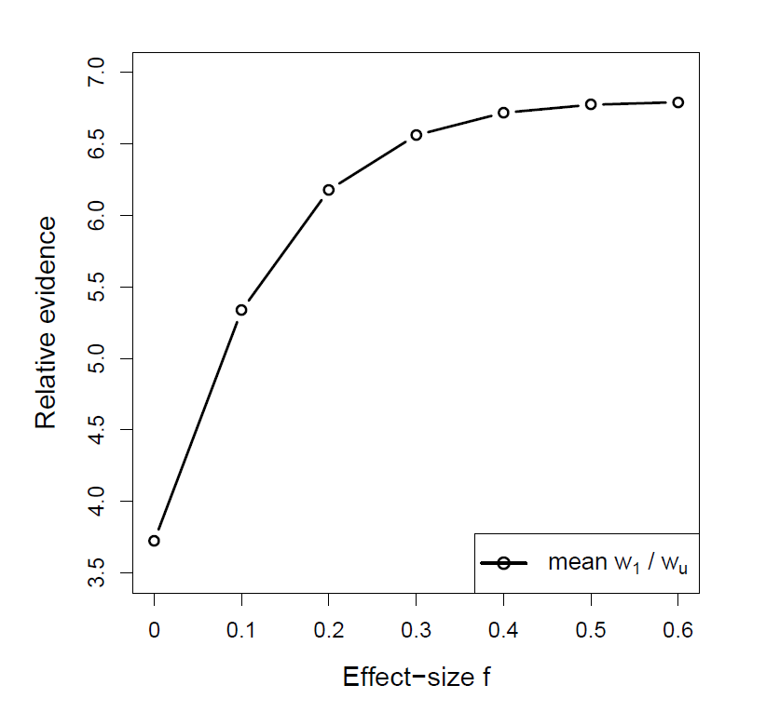
\includegraphics[scale = 0.2]{MaxWeigth.png}\\
		\caption{IC weights can have an upper bound, when informative hypothesis has maximum fit (i.e., is fully in agreement with the data).}
	\end{figure}
\end{frame}
%------------------------------------------------------------------------------%
%
\begin{frame}{Alternative safeguard: Complement of $H_m$}%{using GORIC}
	
	\begin{block}{Alternatively (in case of one hypothesis of interest)}
		Evaluate hypothesis of interest against its complement.\\
		\vspace{\baselineskip}
		More powerful than against the unconstrained \\
		if $H_m$ has maximum fit (which can lead to an upper bound for the GORIC weights).
	\end{block}
	
	\vspace{\baselineskip}
	
	\footnotesize{
		Reference:\\
		Vanbrabant, L., Van Loey, N., \& Kuiper, R. M. (2020). Evaluating a Theory-Based Hypothesis Against Its Complement Using an AIC-Type Information Criterion With an Application to Facial Burn Injury. Psychological Methods, 25(2), 129-142. https://doi.org/10.1037/met0000238
	}
\end{frame}
%------------------------------------------------------------------------------%
%
\begin{frame}{Alternative safeguard: Complement of $H_m$}%{using GORIC}
	%\begin{figure}
	%    \centering
	%  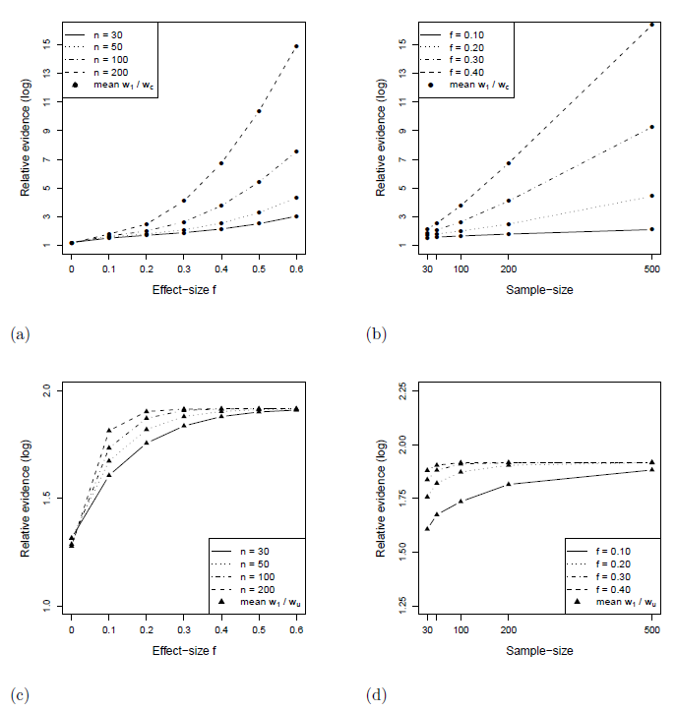
\includegraphics[scale = 0.35]{Weigth_Compl_and_Hu.png}\\
	%  %\caption{IC weights for H1 vs its complement is more powerful when informative hypothesis has maximum fit (i.e., is fully in agreement with the data).}
	%\end{figure}
	\parbox[h]{0.31\textwidth}{
		vs complement\\
		\\
		\\
		\\
		\\
		\\
		\\
		vs unconstrained
	}
	\parbox[h]{0.68\textwidth}{
		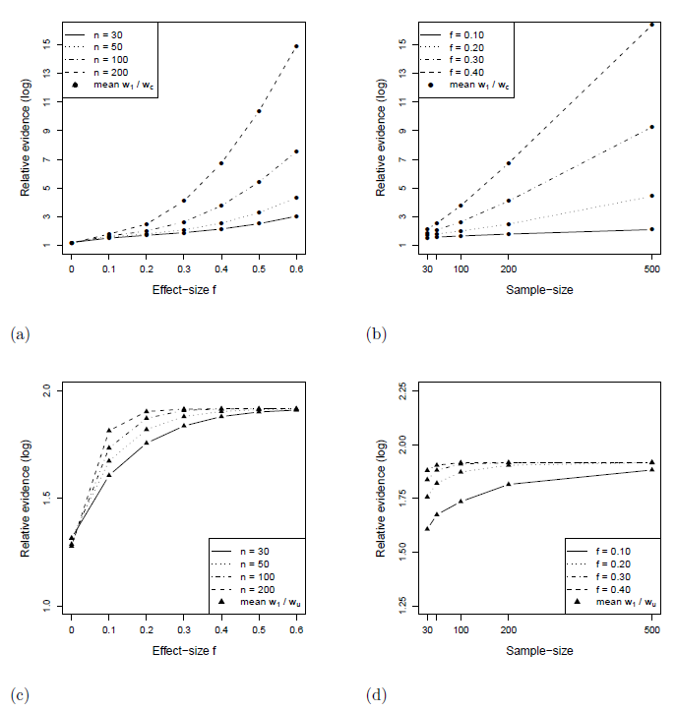
\includegraphics[scale = 0.35]{Weigth_Compl_and_Hu.png}
	}
\end{frame}
%------------------------------------------------------------------------------%
%
\begin{frame}
	\frametitle{Note: complement not always higher weight}
	
	In case $H_m$ is almost true, but not true:
	\begin{enumerate}
		\item $H_m$ does not have maximum fit (but much lower penalty).
		\item Support for $H_m$ is less when evaluating it against its complement (than $H_u$).
	\end{enumerate}
	This is of course a good thing, since $H_m$ is not true.
	
	\vspace{\baselineskip}
	
	Explanation:\\
	Penalty of $H_c$ is smaller than that of $H_u$.\\
	Against $H_u$, you choose $H_m$ 'sooner` because of low penalty for $H_m$.
\end{frame}
%------------------------------------------------------------------------------%
%
\begin{frame}[fragile]{Example: Multigroup regression - model comparison}

\begin{knitrout}
\definecolor{shadecolor}{rgb}{0.969, 0.969, 0.969}\color{fgcolor}\begin{kframe}
\begin{alltt}
\hlkwd{set.seed}\hlstd{(}\hlnum{100}\hlstd{)}
\hlstd{results_MGregr_compl} \hlkwb{<-} \hlkwd{goric}\hlstd{(fit_MGregr,}
                              \hlkwc{hypotheses} \hlstd{=} \hlkwd{list}\hlstd{(H1),}
                              \hlkwc{comparison} \hlstd{=} \hlstr{"complement"}\hlstd{,}
                              \hlkwc{standardized} \hlstd{= T)}
\hlcom{#results_MGregr_compl$result # Output too long for the slide}
\hlstd{results_MGregr_compl}\hlopt{$}\hlstd{result}\hlopt{$}\hlstd{gorica.weights}
\end{alltt}
\begin{verbatim}
## [1] 0.6219892 0.3780108
\end{verbatim}
\begin{alltt}
\hlstd{results_MGregr_compl}\hlopt{$}\hlstd{ratio.gw[}\hlnum{1}\hlstd{,}\hlnum{2}\hlstd{]}
\end{alltt}
\begin{verbatim}
## [1] 1.645427
\end{verbatim}
\end{kframe}
\end{knitrout}

$H_1$ is $.622/.378 \approx 1.645$ times more supported than its complement.\\
Thus, there is only little evidence that $H_1$ is the best of this set.\\
I would now explore for a competing hypothesis for next research...

\end{frame}
%------------------------------------------------------------------------------%
%
\begin{frame}[fragile]{Use of unconstrained and complement}

In case of 1 hypothesis of interest:\\
Use the complement.\\
It acts as another competing (non-overlapping) hypothesis.\\
~\\
In case of 2 or more hypotheses of interest:\\
Use the complement of the set, but this is not yet possible in the software.\\
So, use the unconstrained as failsafe.\\
This is used to check whether at least one of the hypothesis is not weak.\\
Then, the non-weak hypotheses can be compared to all other.

\end{frame}
%------------------------------------------------------------------------------%
%
%------------------------------------------------------------------------------%
\section{Extra} 
%------------------------------------------------------------------------------%
%
%------------------------------------------------------------------------------%
%
\begin{frame}{Contact}

\begin{block}{Websites}
\url{https://github.com/rebeccakuiper/Tutorials}
\url{www.uu.nl/staff/RMKuiper/Software}\\
\url{www.uu.nl/staff/RMKuiper/Websites\%20\%2F\%20Shiny\%20apps}\\
\url{informative-hypotheses.sites.uu.nl/software/goric/}
\end{block}

\begin{block}{E-mail}
r.m.kuiper@uu.nl
%\usepackage{hyperref}
%\href{mailto:exmaple@example.com}{exmaple@example.com}
\end{block}
%\textcolor{gray}{}

\end{frame}
%------------------------------------------------------------------------------%
%
\begin{frame}
	\frametitle{Confirmatory methods - some of my references}
	
	\footnotesize{
		\begin{itemize}
			%\item Anraku, K. (1999). An information criterion for parameters under a simple order restriction. \emph{Biometrika, 86}, 141--152. (ORIC)\\
			\item Kuiper, R. M., and Hoijtink, H. (2010). Comparisons of Means Using Exploratory and Confirmatory Approaches. \emph{Psychological Methods, 15(1)}, 69--86.\\
			\item Kuiper, R. M., Klugkist, I., and Hoijtink, H. (2010). A Fortran 90 Program for Confirmatory Analysis of Variance. \emph{Journal of Statistical Software, 34(8)}, 1--31.\\
			\item Kuiper, R.M., Hoijtink, H. and Silvapulle, M.J. (2011). An Akaike type information criterion for model selection under inequality constraints. \emph{Biometrika, 98}, 495-501. (GORIC)\\
			\item Kuiper, R.M., Nederhof, T., and Klugkist, I. (2015). Properties of hypothesis testing techniques and (Bayesian) model selection for exploration-based and theory-based (order-restricted) hypotheses. \emph{British Journal of Mathematical and Statistical Psychology, 68(2)}, 220 -- 245. \\
			\item 	Alt{\i}n{\i}\c{s}{\i}k, Y., Van Lissa, C. J., Hoijtink, H., Oldehinkel, A. J., and Kuiper, R. M. (2021). Evaluation of inequality constrained hypotheses using a generalization of the AIC. Psychological Methods, 26(5), 599-621. \url{https://doi.org/10.1037/met0000406} (GORICA)
		\end{itemize}
	}
\end{frame}
%------------------------------------------------------------------------------%
%
\begin{frame}
	\frametitle{Note on possibilities multiple studies}
	
	\begin{itemize}
		%\item Update GORIC(A) and GORIC(A) weights.\\
		%More data collected: one can (re-)calculate the GORIC(A) weights.
		\item Update hypotheses. \\
		First data set (or a part of it) generates one or more hypotheses.\\
		Then, other(s) used to determine evidence for that/those.
		\item Aggregate evidence for hypotheses.\\
		Aggregate the support for theories (diverse designs allowed).\\
		Note: Meta-analysis aggregates parameter estimates or effect sizes which need to be comparable. 
	\end{itemize}
	
\end{frame}
%------------------------------------------------------------------------------%
%
%------------------------------------------------------------------------------%
\section{The end}
%------------------------------------------------------------------------------%
%
%------------------------------------------------------------------------------%
%
\begin{frame}{Summary}

  \begin{itemize}
      \item IC
      \item AIC in R
      \item IC weights
      \item GORICA in R
      \item Complement
  \end{itemize}
  
  \vspace*{5mm}
  
  Exploratory vs confirmatory.

\end{frame}
% %------------------------------------------------------------------------------%
% %
% \begin{frame}{Take home message}
% \begin{itemize}
% \item{} 
%   \begin{itemize}
%   \item{}
%   \item{}
%   \end{itemize}
% \item{}
% \end{itemize}
% \end{frame}
%------------------------------------------------------------------------------%
%
\begin{frame}{Thanks \& How to proceed}

Thanks for listening!

\vspace*{5mm}

Are there any questions?\\
\begin{itemize}
  \item Ask fellow participant on course platform.
  \item Ask teacher during Q\&A (or via course platform).
  \item See if making the lab exercises help.
  \item Check a GORICA article or a GORICA tutorial: e.g., \url{https://github.com/rebeccakuiper/Tutorials}.
\end{itemize}

\vspace*{5mm}

You can start working on the lab exercises. % to evaluate theory-based hypotheses using the GORICA

\end{frame}
%------------------------------------------------------------------------------%
%
%------------------------------------------------------------------------------%
%
\end{document}









